% =========================================================================
% Appendix B: Laboratory plate gallery
% =========================================================================

\chapter{Laboratory photographs}
\label{app:plate_gallery}

These plates document culture and assay work. Captions name only marks that are visible on the lid or disc. Unlabelled assay plates are not assigned to a species. MET~5 discs are not the gentamicin control used in the tabulated assays.

\section{Labelled cultures}
\label{sec:app_cultures}

\begin{figure}[hbt!]
  \centering
  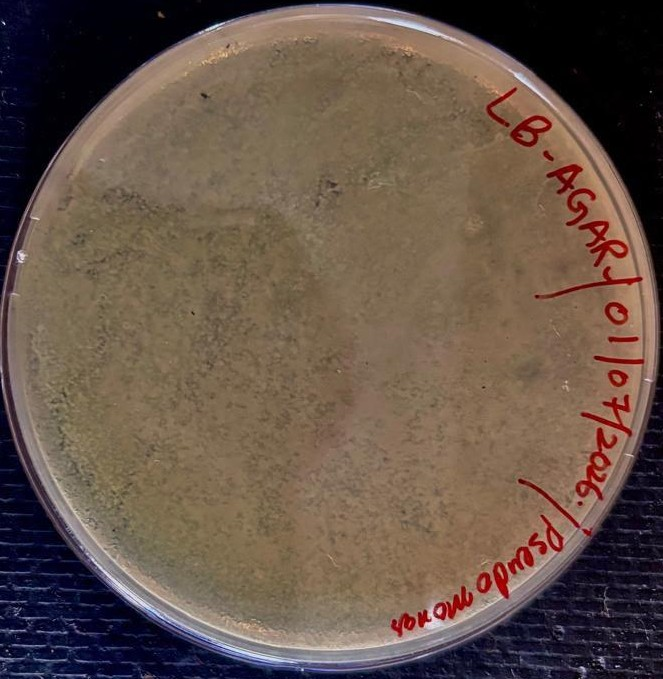
\includegraphics[width=0.62\textwidth]{figures/fig_paeruginosa_culture.jpg}
  \caption{LB agar culture labelled \textit{Pseudomonas}, 01-07-2026. This is a culture plate, not an inhibition assay.}
  \label{fig:paeruginosa_culture}
\end{figure}

\begin{figure}[hbt!]
  \centering
  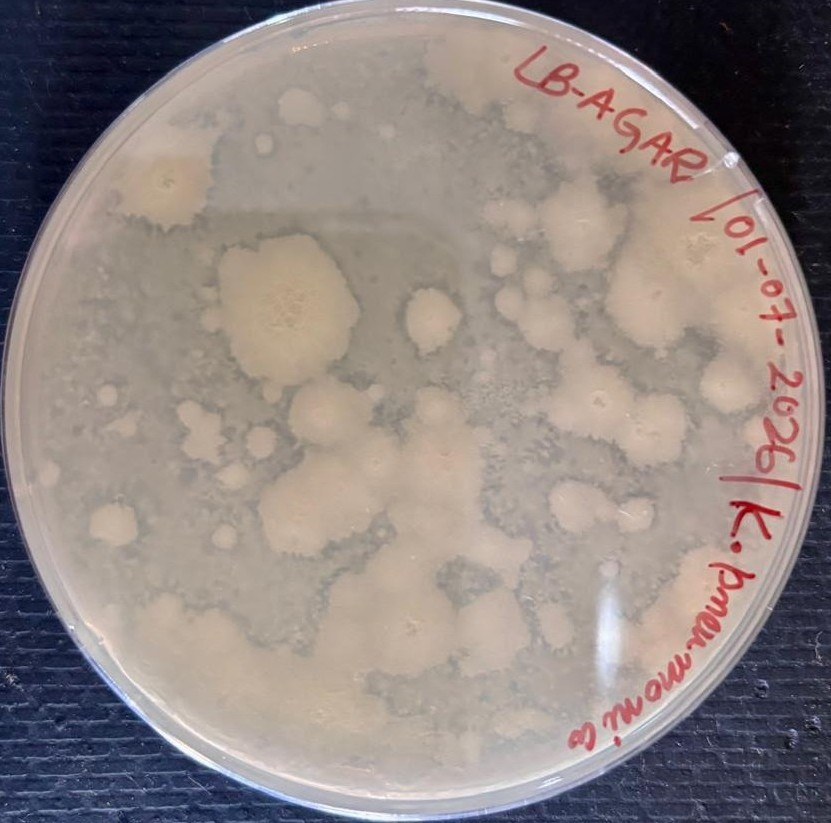
\includegraphics[width=0.62\textwidth]{figures/fig_kpneumoniae_culture.jpg}
  \caption{LB agar culture labelled \textit{K.\ pneumoniae}, 01-07-2026. This is a culture plate, not an inhibition assay.}
  \label{fig:kpneumoniae_culture}
\end{figure}

\begin{figure}[hbt!]
  \centering
  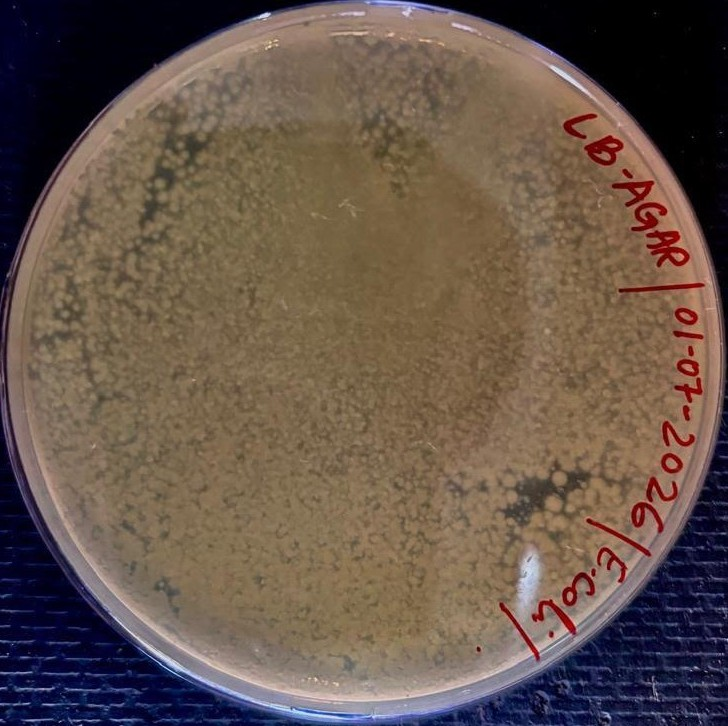
\includegraphics[width=0.62\textwidth]{figures/fig_ecoli_culture_b.jpg}
  \caption{LB agar culture labelled \textit{E.\ coli}, 01-07-2026.}
  \label{fig:ecoli_culture_b}
\end{figure}

\begin{figure}[hbt!]
  \centering
  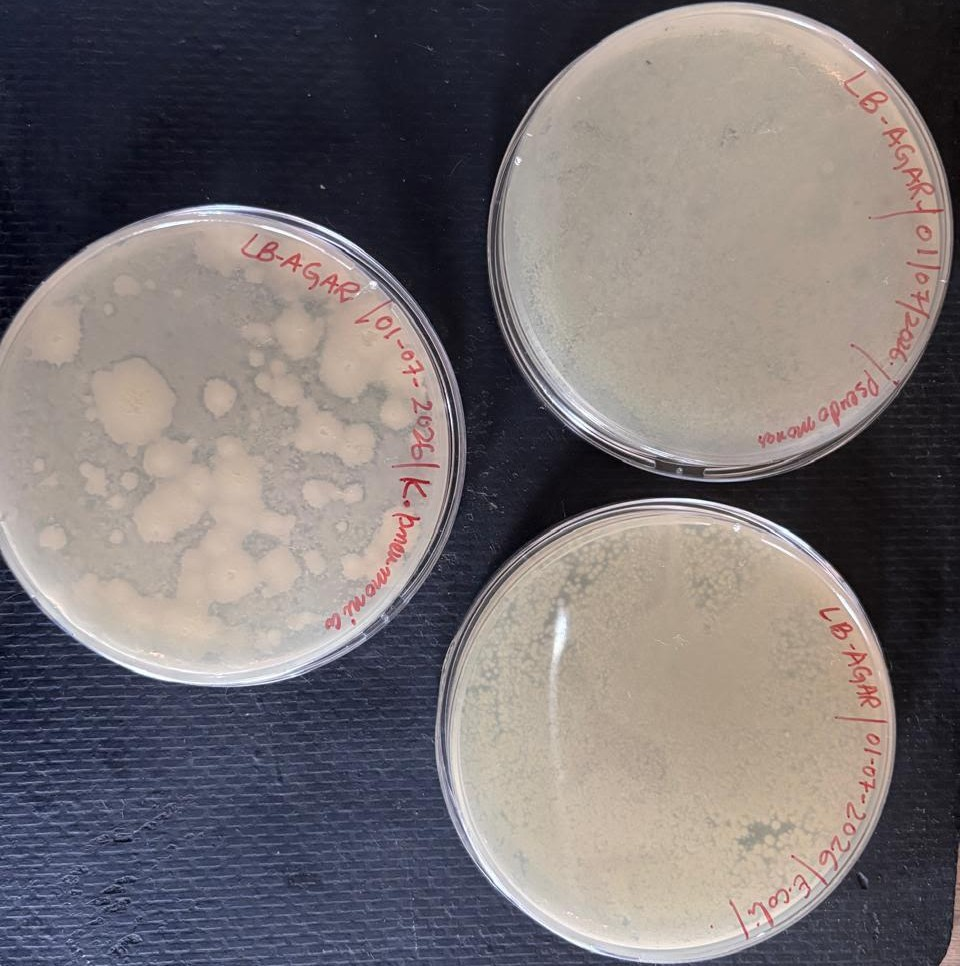
\includegraphics[width=0.78\textwidth]{figures/fig_three_cultures_labelled.jpg}
  \caption{Three LB agar cultures (01-07-2026) labelled \textit{K.\ pneumoniae}, \textit{Pseudomonas}, and \textit{E.\ coli}.}
  \label{fig:three_cultures_labelled}
\end{figure}

\section{Assay plates without a species name on the lid}
\label{sec:app_unlabelled_assays}

\begin{figure}[hbt!]
  \centering
  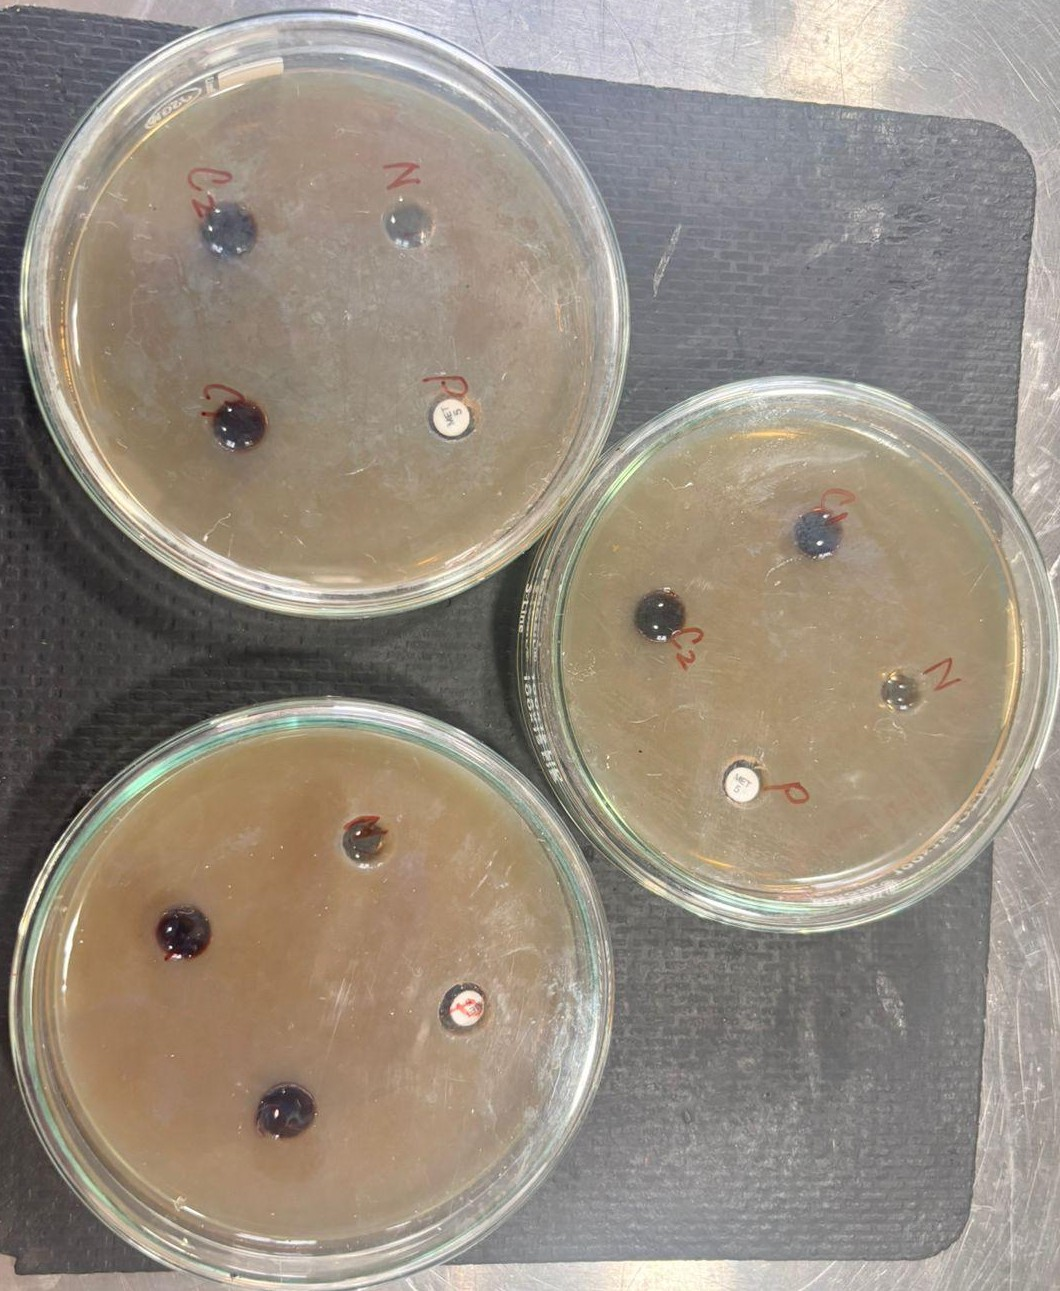
\includegraphics[width=0.78\textwidth]{figures/fig_assay_trio_unlabelled.jpg}
  \caption{Three well-and-disc plates. Wells are marked C1, C2, and N; discs are commercial gentamicin. The lids do not name the organism.}
  \label{fig:assay_trio_unlabelled}
\end{figure}

\begin{figure}[hbt!]
  \centering
  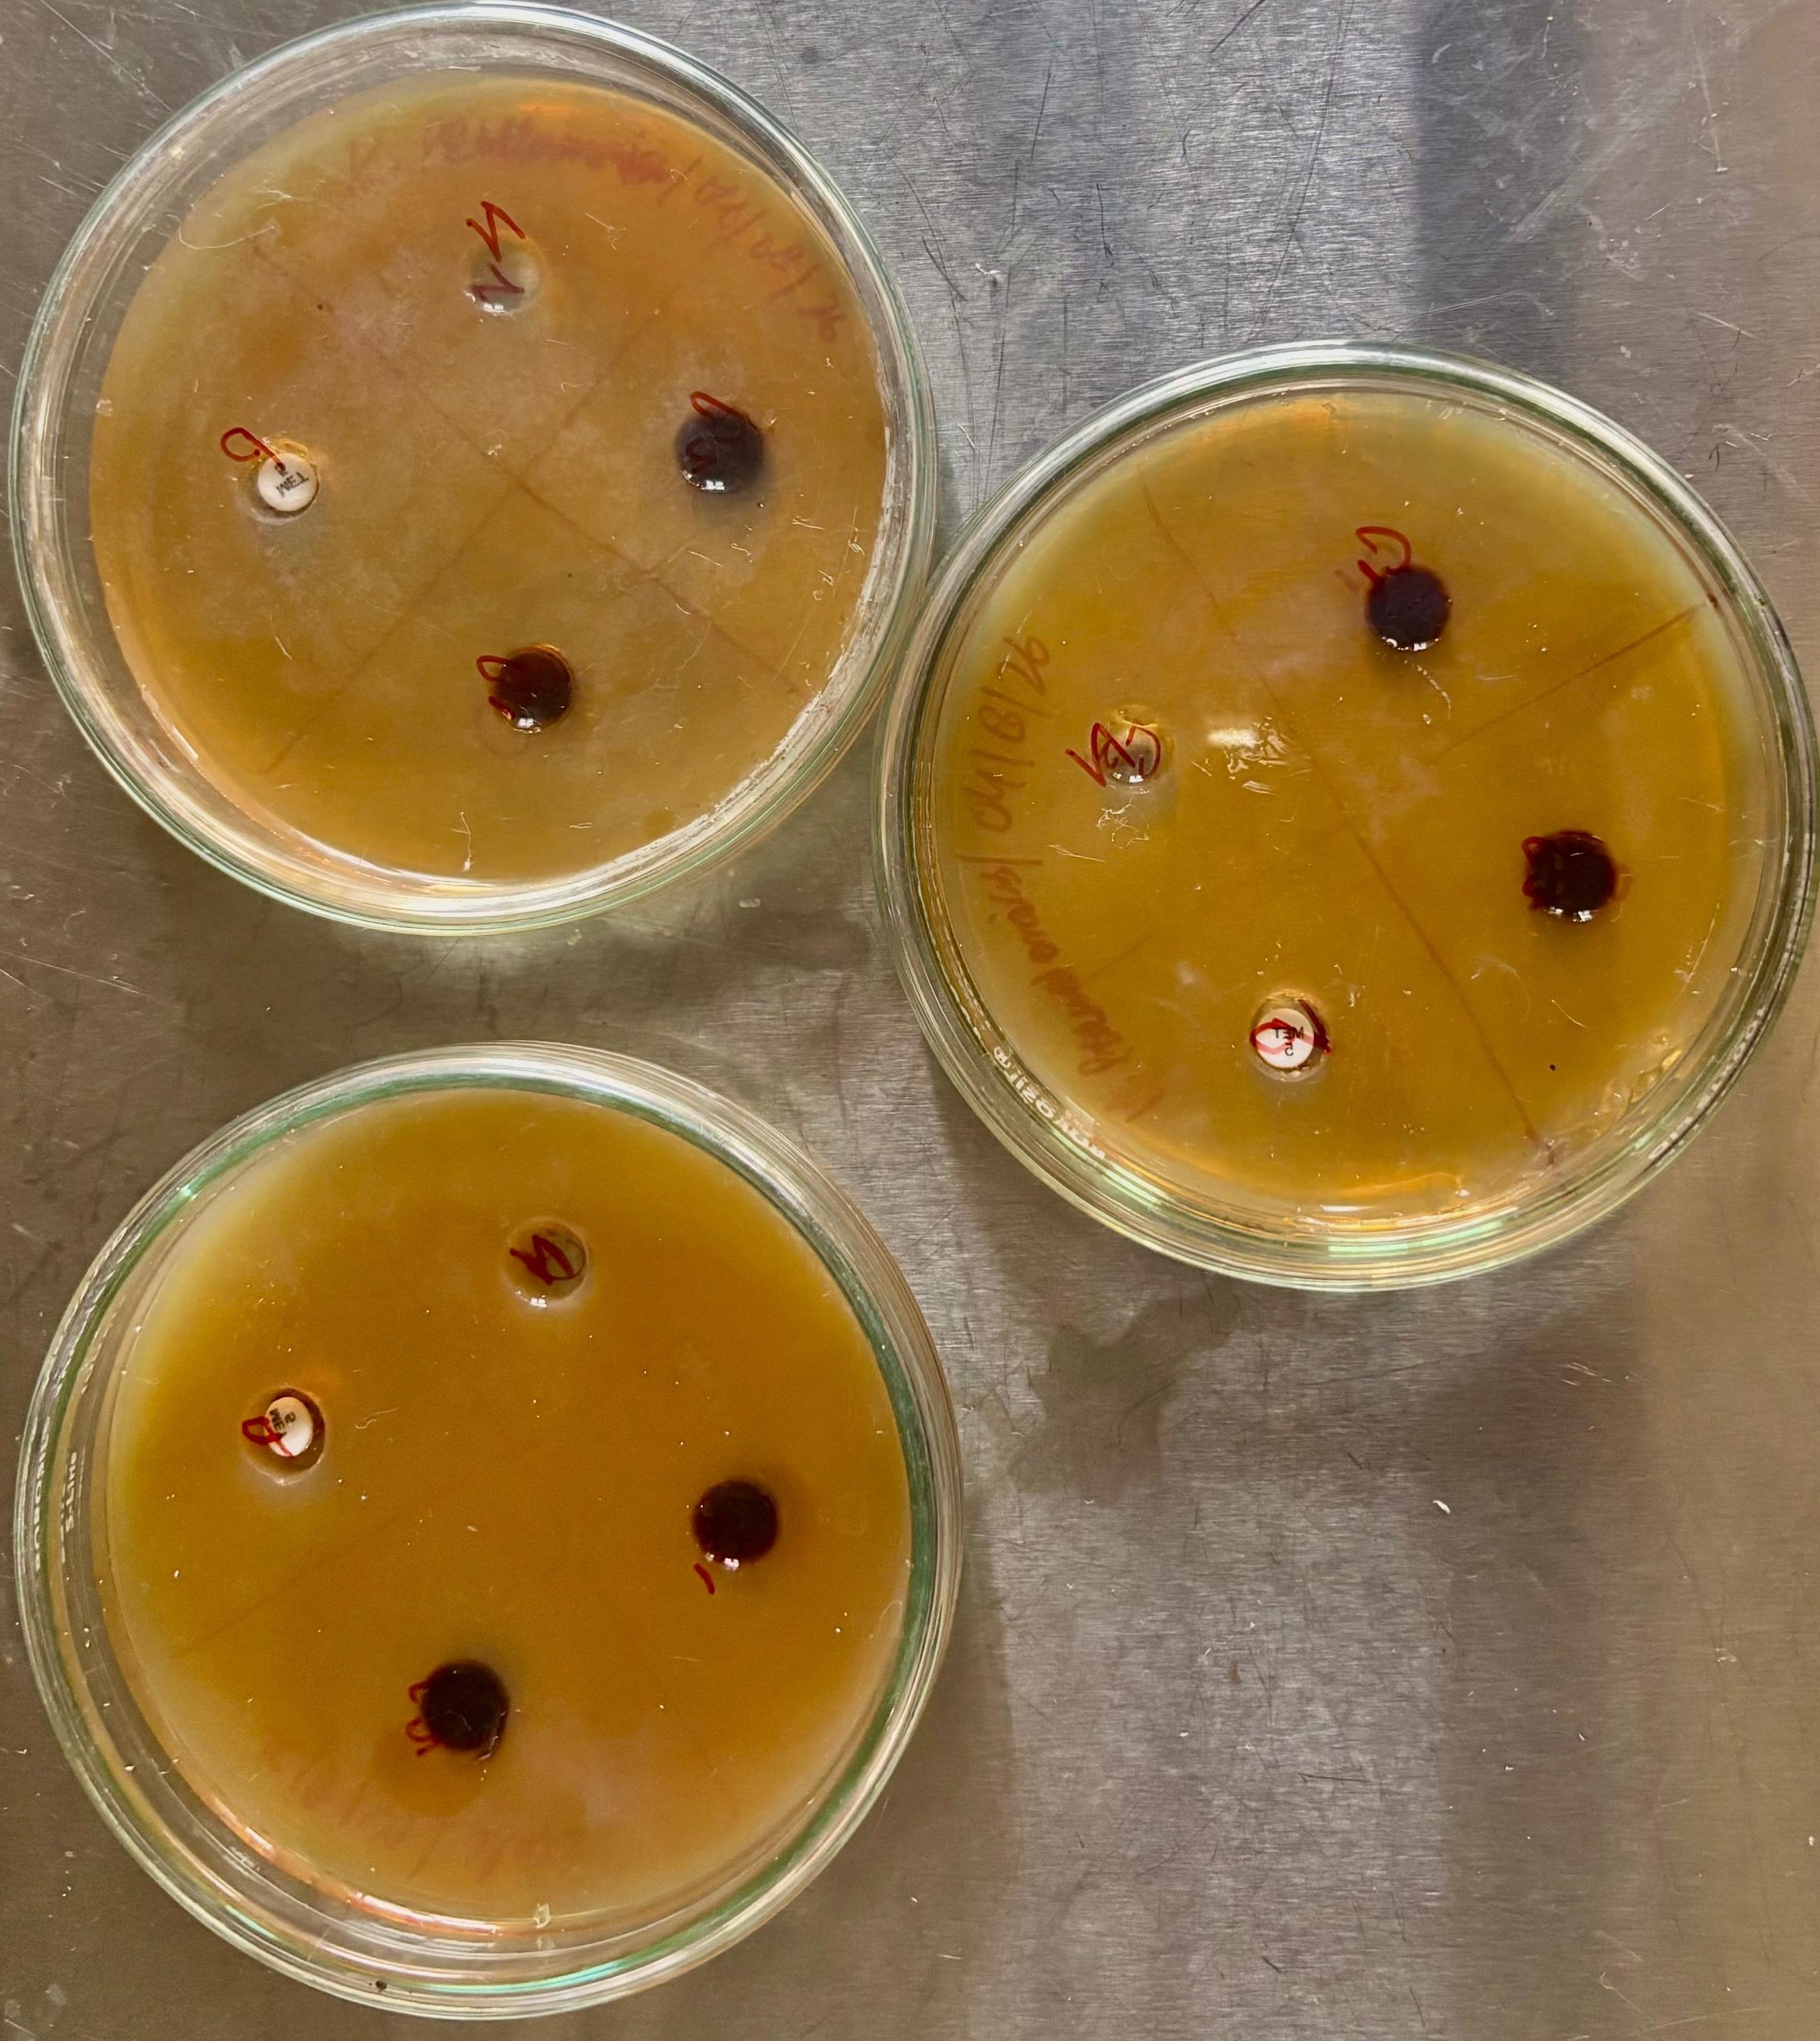
\includegraphics[width=0.78\textwidth]{figures/fig_assay_trio_dated.jpg}
  \caption{Three assay plates dated 04/8/26. One lid is marked \textit{K.\ pneumoniae}; the other two lids are not used here as species identifications.}
  \label{fig:assay_trio_dated}
\end{figure}

\begin{figure}[hbt!]
  \centering
  \begin{minipage}[t]{0.48\textwidth}
    \centering
    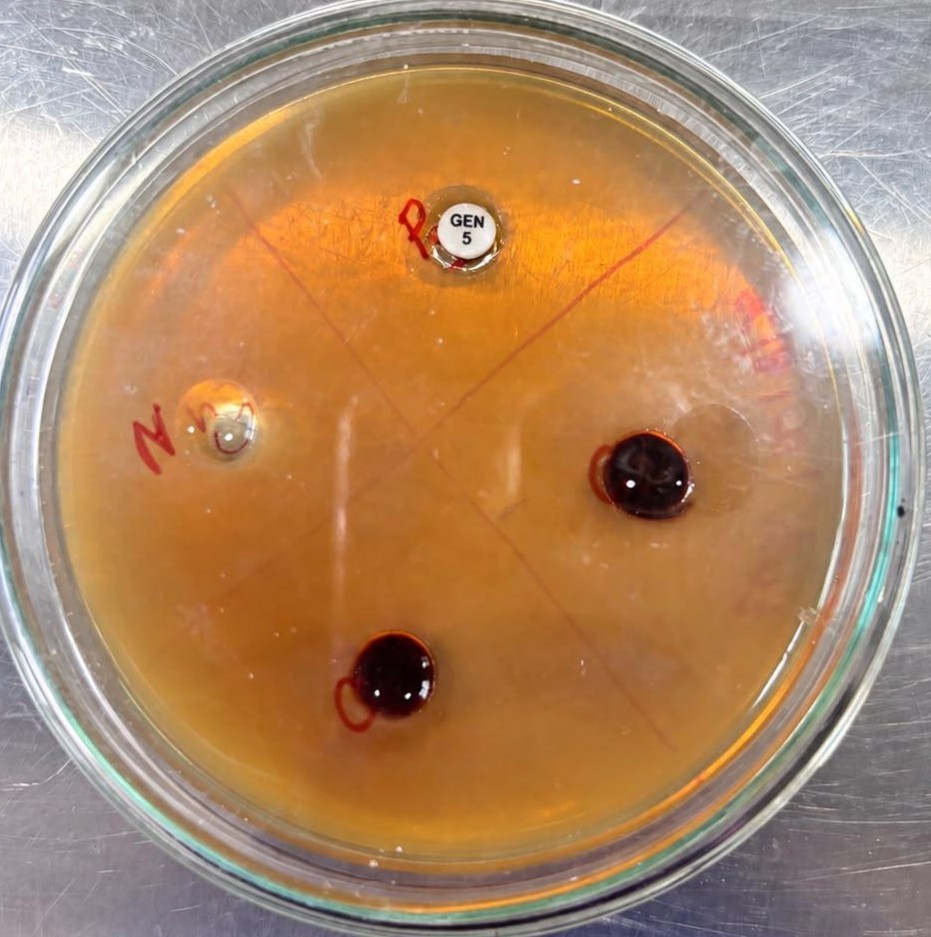
\includegraphics[width=\linewidth]{figures/fig_gen5_unlabelled_b.jpg}
    \caption{Well-and-disc plate. Disc labelled GEN~5; wells N and extract. Organism not named on the lid.}
    \label{fig:gen5_unlabelled_b}
  \end{minipage}
  \hfill
  \begin{minipage}[t]{0.48\textwidth}
    \centering
    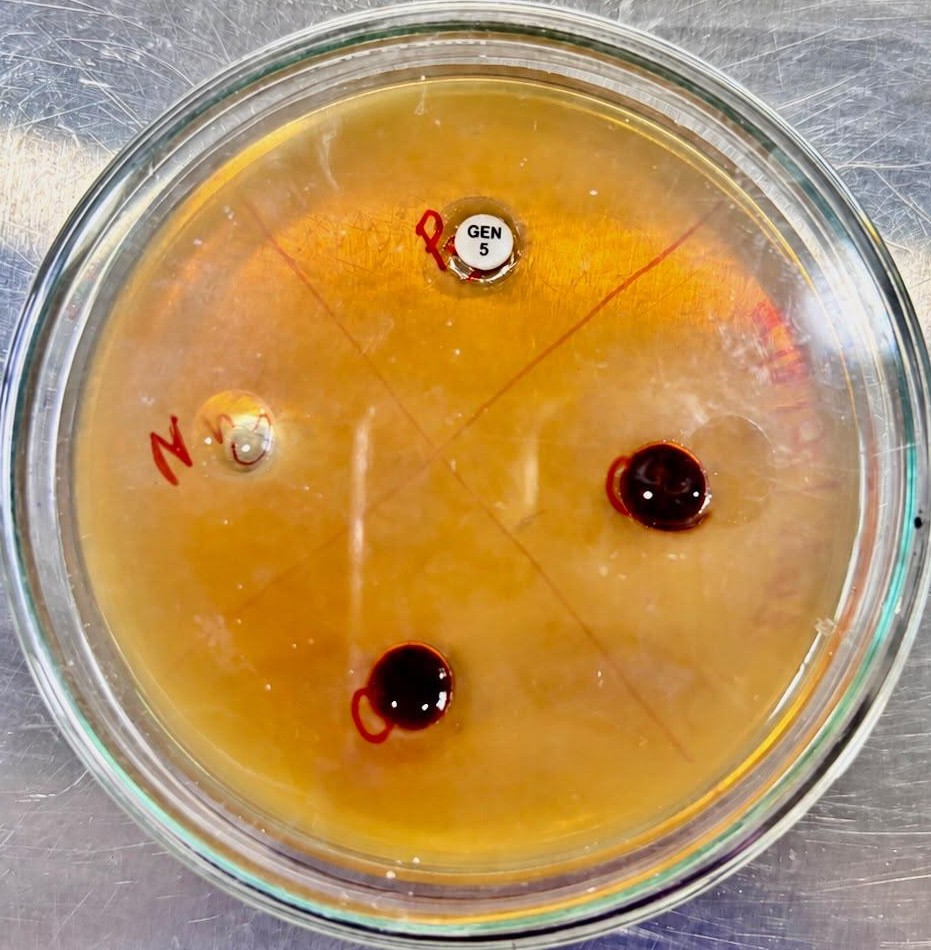
\includegraphics[width=\linewidth]{figures/fig_gen5_unlabelled_c.jpg}
    \caption{Second GEN~5 well-and-disc plate. Organism not named on the lid.}
    \label{fig:gen5_unlabelled_c}
  \end{minipage}
\end{figure}

\begin{figure}[hbt!]
  \centering
  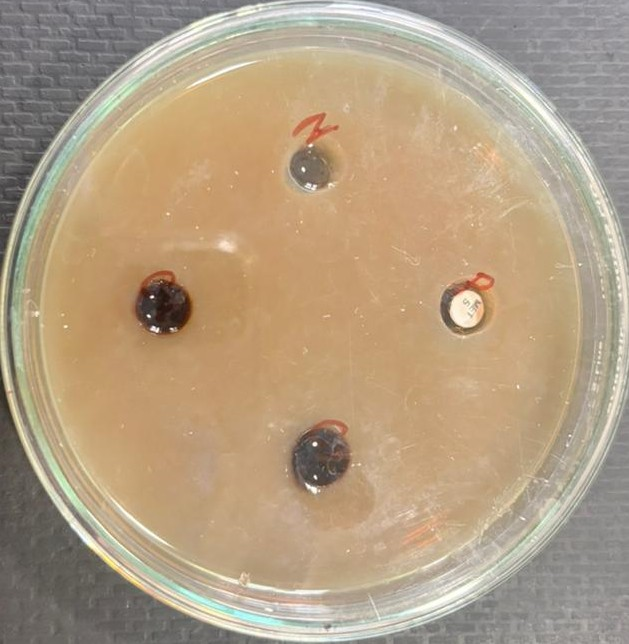
\includegraphics[width=0.55\textwidth]{figures/fig_gen_unlabelled_close.jpg}
  \caption{Close view of a well-and-disc plate. Disc marked GEN; wells N and extract. Organism not named.}
  \label{fig:gen_unlabelled_close}
\end{figure}

\begin{figure}[hbt!]
  \centering
  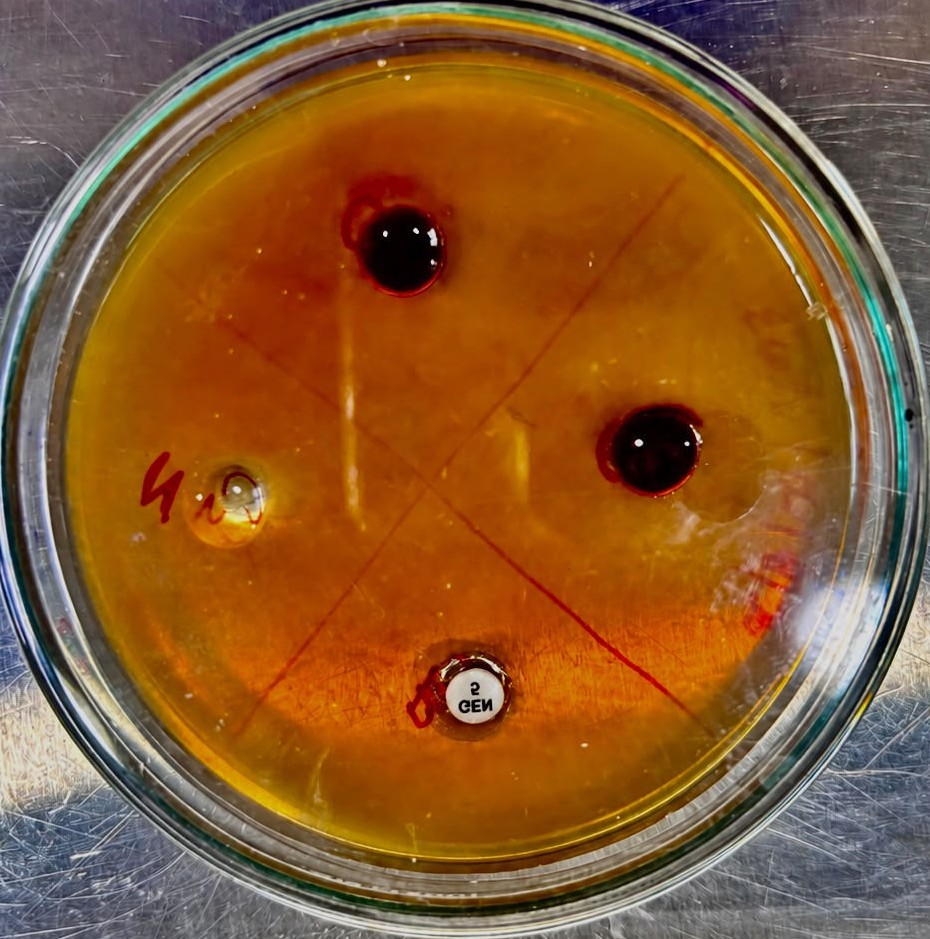
\includegraphics[width=0.55\textwidth]{figures/fig_gen2_unlabelled.jpg}
  \caption{Well-and-disc plate. Disc labelled GEN~2; wells N and extract. Organism not named. This disc is not the GEN~5 control used in the tabulated series.}
  \label{fig:gen2_unlabelled}
\end{figure}

\begin{figure}[hbt!]
  \centering
  \begin{minipage}[t]{0.48\textwidth}
    \centering
    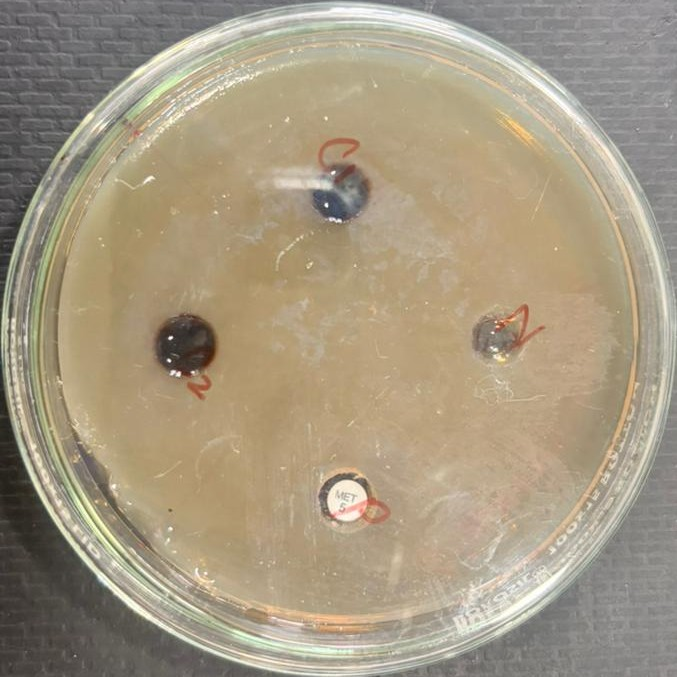
\includegraphics[width=\linewidth]{figures/fig_met5_unlabelled_a.jpg}
    \caption{Assay plate with a disc labelled MET~5 and wells marked C and N. Organism not named. MET~5 is not the tabulated gentamicin control.}
    \label{fig:met5_unlabelled_a}
  \end{minipage}
  \hfill
  \begin{minipage}[t]{0.48\textwidth}
    \centering
    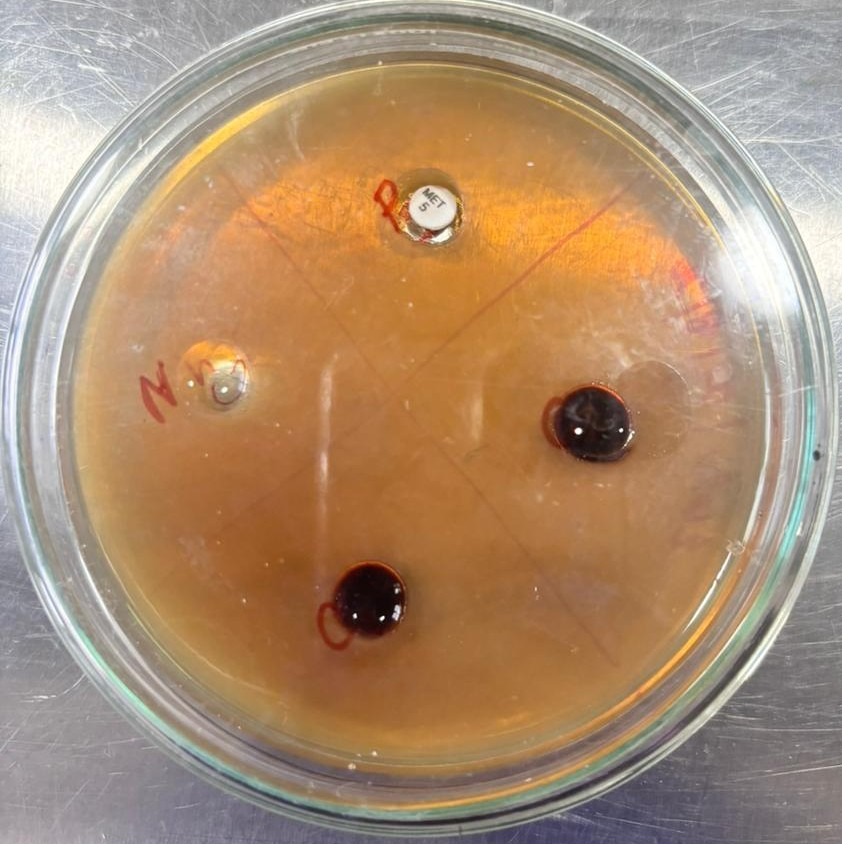
\includegraphics[width=\linewidth]{figures/fig_met5_unlabelled_b.jpg}
    \caption{Second MET~5 well-and-disc plate. Organism not named.}
    \label{fig:met5_unlabelled_b}
  \end{minipage}
\end{figure}
